\chapter{Adventuring}
\label{ch:adventuring}


\section{Spot Rules}
This selection of rules is designed to deal with individual situations that may crop up throughout the game. 

\subsection{Travel}

The rates given below are based on average movement rates. If you need to precisely determine which of two groups reached a destination first, use an Opposed Athletics (for walking) or Riding test.
\begin{table}[h]
\begin{center}
\caption{Daily Travel Rates}
\label{tab:daily-travel-rates}
\begin{rpg-table}[|l|c|X|]
        \hline
	\textbf{Type} & \textbf{Rate/day} & \textbf{Notes}\\
        \hline
	Hiking          & 50km   & Ten hours of steady walking on road or path with no wagons or animals. Need to make Fatigue Test at the end of the Hike to avoid becoming Fatigued.\\
	Marching        & 30km   & Marching in organised groups for ten hours, ready to fight at the end of the day. No need for a Fatigue test at the end of the march.\\
	Riding Slow     & 30km   & Moving at a walk accompanied by pack animals and wagons.\\
	Riding          & 50km   & Casual riding.\\
	Riding Fast     & 90km   & Riding fast with no wagons. Both mount and rider need to make a Fatigue test at the end of the day.\\
        \hline
\end{rpg-table}
\end{center}
\end{table}

The above rates should also be modified by the type of terrain being crossed.

\begin{rpg-table}[|X|Y|]
        \hline
	\textbf{Terrain} & \textbf{Movement Adjustment}\\
        \hline
	Road/Path                & 100\% of normal rate\\
	Light brush              & 80\% of normal rate\\
	Medium brush             & 70\% of normal rate\\
	Light woods              & 70\% of normal rate\\
	Rolling Hills            & 70\% of normal rate\\
	Heavy woodland           & 50\% of normal rate\\
        \hline
\end{rpg-table}


\subsection{Illumination \& Darkness}
Table~\ref{tab:illumination-and-darkness} gives examples of several different levels of illumination and darkness and the effects/penalties that it may have on the characters.
\begin{table*}
\begin{center}
\caption{Illumination \& Darkness}
\label{tab:illumination-and-darkness}
\begin{rpg-table}[|c|X|X|]
        \hline
	\textbf{Environtment} & \textbf{Example} & \textbf{Effects}\\
        \hline
	Brightly Illuminated & Blazing summer day  & None.\\
	Illuminated          & Heavy candlelit room, overcast day, within radius of illuminating item & None.\\
	Partial Darkness     & Cavern mouth, misty day, within 3 x radius of illuminating item (see below). & -20\% to vision-based Perception tests and combat attacks.\\
	Darkness             & Large cavern illuminated only by embers, foggy day, within 5 x radius of illuminating item. & -40\% to vision-based Perception tests and combat attacks. Movement rate halved.\\
	Pitch Black          & Sealed room with stone walls, cavern many miles underground, supernatural darkness, mountaintop whiteout. & Perception tests reliant on vision become near impossible, as are ranged attacks. Close combat attacks are at -60\%. Movement rate a quarter of normal.\\
        \hline
\end{rpg-table}
\end{center}
\end{table*}

%\subsubsection{Dark Sight}
%This allows the character to treat pitch black conditions as if dark. Normally possessed by subterranean or darkness aligned creatures.

\subsubsection{Night Vision}
This allows the character to see at night as well as during the day. Normally possessed by subterranean or darkness aligned creatures.

\subsubsection{Night Sight}
This ability allows the character to treat partial darkness as illuminated and darkness as only partial darkness. This is normally possessed by nocturnal creatures.

\subsubsection{Blind Sight}
The ability of some animals to fight as if sighted although they are not. For example, using ground vibrations, echolocation, acute hearing or scent. The exact reason would typically be described in parenthesis, e.g. Blind Sight (Echolocation).


\subsection{Fatigue}
Combat, sprinting, climbing, swimming against a strong current, are all examples of when a character can become fatigued and tired.

If the Gamemaster thinks that a character has been engaged in an activity that may have drained him of physical energy, then they may call for a Resilience roll. If the character fails the roll they suffer the effects of Fatigue.

\begin{rpg-examplebox}
Rurik has just been in a long, ten round, combat against a group of bandits. Although he has emerged victorious, the Gamemaster rules that Rurik has to roll a successful Resilience test or become Fatigued.
\end{rpg-examplebox}

This test is usually made after the activity has been completed, unless the activity is long and drawn out and there is a real danger that Fatigue will stop the task being completed successfully. For example, on a long hard march the characters are pressing on ahead so that they can reach a fort before an enemy army arrives there. In this case there is a real danger that they will arrive not only too late but tired and worn down.

\begin{figure}%[h]
\begin{center}
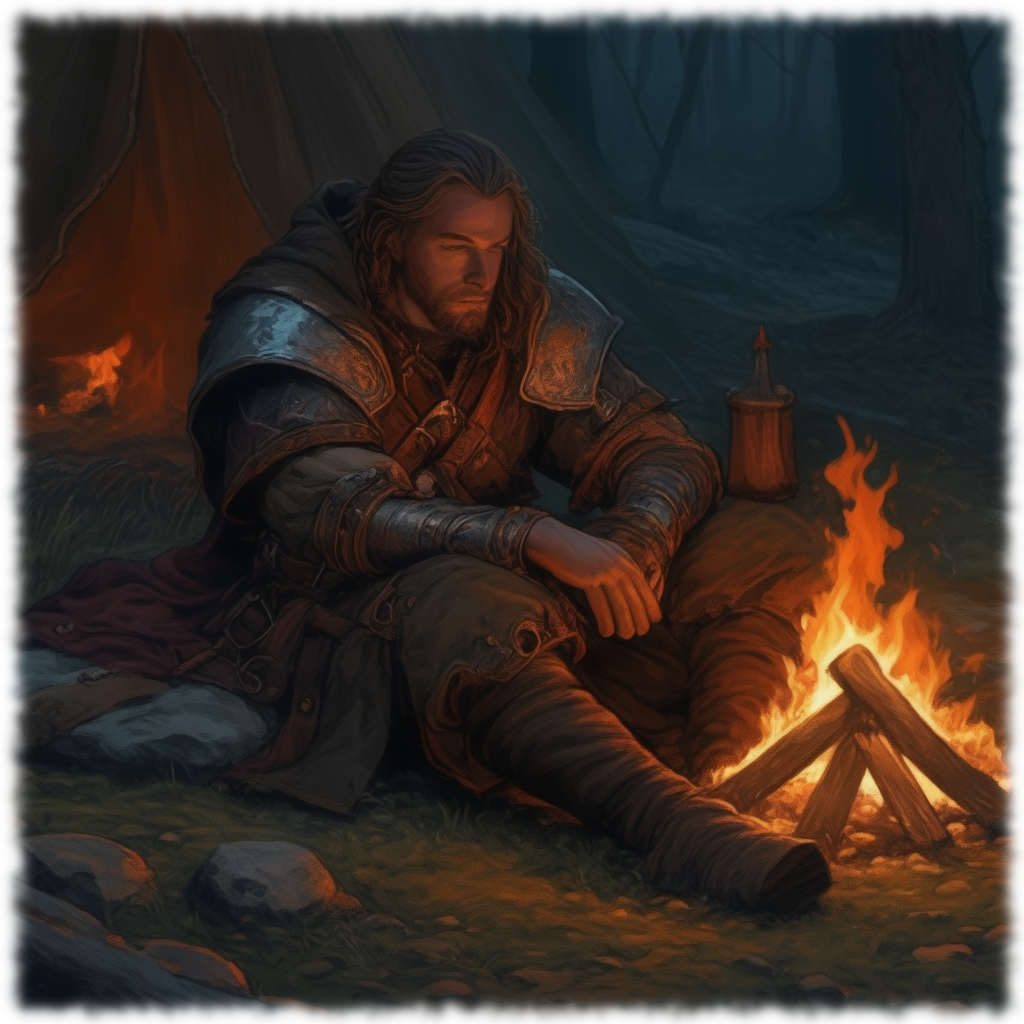
\includegraphics[scale=0.24]{img/ai-images/fatigue.png}
\end{center}
\end{figure}

\begin{table}
\begin{center}
\caption{Illuminating Items}
\label{tab:illuminating-items}
\begin{rpg-table}[|X|Y|]
        \hline
	\textbf{Example} & \textbf{Radius}\\
        \hline
	Candle or embers      & 1m\\
	Torch or lantern      & 3m\\
	Campfire              & 5m\\
	Bonfire               & 10m\\
        \hline
\end{rpg-table}
\end{center}
\end{table}


\subsubsection{The Effects of Fatigue}
If a character fails the Resilience test then they become fatigued. All skill tests are at -20\%. Also movement rate drops by a quarter. The character also becomes sluggish, DEX and INT are each reduced by three points for the purposes of determining Combat Order.

If the fatigued character insists on engaging in heavy activity, such as combat, heavy labour or running, then another Resilience roll is made at -20\%. If the character fails this second skill test they become heavily fatigued and all the above penalties are doubled.

If a character fumbles any of their Resilience rolls, then they immediately fall unconscious for 3D6 minutes and upon waking are still fatigued.

\subsubsection{Recovering from Fatigue}
A character who completely rests for 20-CON hours will remove the effects of any Fatigue. Certain Powers might also help remove the effects of Fatigue.


\subsection{Exposure, Starvation and Thirst}

\subsubsection{Exposure}
A character can normally survive for a number of hours equal to his CON before suffering from exposure. 

\subsubsection{Starvation}
A character can survive for a number of days equal to his CON before becoming starved, though after three days they will begin to suffer a –10\% penalty to Fatigue tests. 

\subsubsection{Thirst}
A character can survive for a number of hours equal to his CON x 2 before becoming chronically thirsty, though particularly arid environments may reduce this to CON x 1 or even CON x 1/2. 

\subsubsection{Effects and Remedy}
Whenever a character is suffering from exposure, starvation or thirst, a Fatigue test penalty is required with a -20\%. In addition, the character will automatically suffer one 1D6 of damage every day, for every condition he is experiencing. Natural healing will not heal this damage – only sufficient shelter, food or water can remedy the problem and allow natural healing to take place. 


\subsection{Healing}
Healing can be performed in one of two ways – using the First Aid skill or through natural healing, resting while the injuries heal themselves. 

\subsection{Natural Healing}
A character’s Minor injuries regain CON/4 (round up) hit point per 24 hours, as long as the character does not engage in anything more than light activity. 

Natural healing will not improve Major Wounds. A Major Wound requires treatment with a successful Healing test. Once this is done Major Wounds heal at a rate of one hit point per day, as long as the character does not engage in anything more than light activity, and the character succeeds a daily Resilience test. 


\subsection{Encumbrance}
\label{ssec:encumbrance}
Every piece of equipment in the Equipment chapter has an Encumbrance (ENC) score, apart from those items that are too small or light. Characters can usually ignore the effects on Encumbrance that these light items have until they start to carry a lot of them – assume that an average of 20 such items will equal 1 ENC, on the basis that the character has a suitable means of carrying them, such as a sack or backpack. 

A character can carry equipment whose total ENC is less than or equal to his STR+SIZ without penalty. 

Encumbrance is a measure of not only weight but also bulk of the item, reflecting the awkwardness of handling the item. Roughly 1 ENC is equal to 1/4 of a SIZ point.

\subsubsection{Overloading}
A character carrying total ENC greater than his STR+SIZ is Overloaded. 
\begin{rpg-list}
\item Overloaded characters suffer a –20\% penalty to all tests that require physical actions, including Weapon skill tests and most tests that have DEX or STR as a Characteristic. 

\item Overloaded characters have their Movement halved. They also suffer a –20\% penalty to all Fatigue tests. 
\end{rpg-list}

A character cannot carry more than twice his STR+SIZ in ENC. 

\subsection{Falling}
\label{ssec:falling}
A character that takes damage from a fall ends up prone. Armour points do not reduce falling damage. 
A character takes 1D6 damage per full 3m fallen.

As long as the character was not surprised, they may attempt an Athletics test to mitigate falling damage. A successful test allows the character to treat the fall as if it were two metres shorter than it actually is. In addition, as long as this test is a success and the character is not reduced to 0 hit points due to the fall, the character lands safely and is not prone. If the roll is a critical then miraculously no damage is taken. If the roll is a fumble then the maximum possible damage is taken.

Characters falling onto soft surfaces may have the distance they fall effectively halved for the purposes of damage. 


\subsection{Suffocation}
\label{ssec:suffocation}
While underwater or moving through a poison gas cloud a character can hold his breath for a number of Combat Rounds equal to his CON. 

Once a character has surpassed the time for which he can hold his breath, he must make a Resilience test every round with a cumulative –10\% penalty. If he fails, he automatically starts inhaling the suffocating substance.

\begin{table}
\begin{center}
\caption{Suffocating Substance}
\label{tab:suffocating-substance}
\begin{rpg-table}[|l|Y|]
        \hline
	\textbf{Substance Inhaled} & \textbf{Damage Taken}\\
        \hline
	Water         & 2D6\\
	Vacuum        & 2D6\\
	Thick Smoke   & 1D6\\
	Poison Gas    & Character is exposed to the poison. If the gas is also a thick smoke, then 1D6 damage is incurred in addition to the poison’s effect.\\
        \hline
\end{rpg-table}
\end{center}
\end{table}

Armour points do not reduce suffocation damage. The damage will only cease once the character can draw breathable air once more. Even then, the character will require a Resilience test to be able to do anything other than wretch or gasp for breath for 1D4 Combat Rounds. 


\subsection{Burning}
The amount of damage per Combat Round suffered from fire or heat will depend on its intensity, as shown on the Fire and Heat Table.%table~\ref{tab:fire-and-heat}. 
Metal armour, such as Plate or Chain mail, does not subtract from the rolled damage.

\begin{table}
\begin{center}
\caption{Fire and Heat}
\label{tab:fire-and-heat}
\begin{rpg-table}[|l|X|l|]
        \hline
	\textbf{Damage Source} & \textbf{Example} & \textbf{Damage/CR}\\
        \hline
	Flame            & Candle       & 1 point\\
	Large Flame      & Torch        & 1D4 points\\
	Small Fire       & Camp fire    & 1D6 points\\
	Large Fire       & Scolding steam, large bonfires, burning rooms & 2D6 points\\
	Inferno          & Lava, inside a blast furnace & 3D6 points\\
        \hline
\end{rpg-table}
\end{center}
\end{table}


\subsection{Poison}
Plants and creatures have developed poisons as a method of protecting themselves against predators. They are also used by assassins and wrong doers of all kinds to murder their victims.  
Every type of poison has the following information detailed: 

\begin{description}
	\item[Name:] The poison’s name. Also, if the poison is not natural, it will be mentioned here. 
	\item[Type:] Lists whether the poison is ingested, used on a weapon, or inhaled. 
	\item[Delay:] The time between the poison’s introduction to a character, to the time its effect takes hold. 
	\item[Potency:] This is a number between 10 and 100 that measures the strength of a poison. Some supernatural poisons, like Basilisk Venom, have even higher Potencies. A character must make an opposed Resilience test versus the poison’s Potency test in order to avoid or mitigate the damage of the poison. 
	\item[Effect:] Usually hit point damage, though this is not universal. Some poisons cause a character to sleep for a period of time. More exotic poisons may cause hallucinogenic effects, paralysis or a combination of effects. These take place after the delay noted above. 
	\item[Duration:] How long the poison, if effective, will affect the victim. The effects of the poison cannot be removed or healed until the poison itself has been neutralised or has dissipated in the victim’s system. Hit point damage caused by poison will recover through natural healing. 
\end{description}

The character's Resilience and the Poison's potency are rolled against each other similar to opposed skill checks.

\subsubsection{Example: Gorgon Serpent Venom}

\noindent\textbf{Type:} Ingested or smeared\\
\noindent\textbf{Delay:} 1D3 Combat Rounds\\
\noindent\textbf{Potency:} 34\\
\noindent\textbf{Effect:} 1D3 hit point damage and -3 penalty to CON\\
\noindent\textbf{Duration:} 6D10 minutes\\

%\begin{description}
%\item[Type:] Ingested or smeared
%\item[Delay:] 1D3 Combat Rounds
%\item[Potency:] 34
%\item[Effect:] 1D3 hit point damage and -3 penalty to CON
%\item[Duration:] 6D10 minutes
%\end{description}

Other poisons: Viper Venom, Belladonna, Mushrooms, Scorpion Sting, Pokeweed or Holly Berries, etc.

\subsection{Disease}
\label{ssec:disease}
Disease is a source of threat in fantasy worlds, either from diseases that ravage the land from time to time or even supernatural diseases.
Every type of disease has the following information detailed: 

\begin{description}
	\item[Name:] The disease’s name. Also, if the disease is not natural, it will be mentioned here. 
	\item[Type:] Lists whether the disease is spread through contamination, touch or is airborne. 
	\item[Delay:] The time between the diseases introduction to a character, to the time its effect takes hold. It is also the time following disease contraction that a victim will be forced to make follow-up opposed disease tests.
	\item[Potency:] This is a number between 10 and 100 that measures the strength of a disease. Some supernatural diseases, like the shining plague, have even higher Potencies. A character must make an opposed Resilience test versus the disease’s Potency test in order to avoid or mitigate the damage of the disease.
	\item[Effect:] Usually hit point damage, though this is not universal. Many diseases will apply a penalty to Characteristics or skills. More exotic diseases may cause hallucinogenic effects, paralysis or a combination of effects. These take place after the delay noted above. 
\end{description}

The effects of the disease cannot be removed or healed until the disease itself has been neutralised or has dissipated in the victim’s system. Hit point damage caused by disease will recover through natural healing.

\subsubsection{Example: The Shakes}

\noindent\textbf{Type:} Touch\\
\noindent\textbf{Delay:} 1-2 days\\
\noindent\textbf{Potency:} 50\\
\noindent\textbf{Effect:} This flu-like disease renders its victims in a cold and constantly shaking state, during which DEX is halved. Also for each day that the victim suffers from the Shakes they take 1D6 hit points of damage.\\

%\begin{description}
%\item[Type:] Touch
%\item[Delay:] 1-2 days
%\item[Potency:] 50
%\item[Effect:] This flu-like disease renders its victims in a cold and constantly shaking state, during which DEX is halved. Also for each day that the victim suffers from the Shakes they take 1D6 hit points of damage.
%\end{description}

Other diseases: Typhoid, Cholera, Leprosy, Rabies, Malaria, Tuperculosis, Trachoma, etc.

\subsection{Inanimate Objects}
All inanimate objects have armour points and hit points. Except in the most unusual of circumstances, attacks on inanimate objects will automatically hit – characters simply need to work out how much damage they deal. 

The object’s armour points will be deducted from any damage dealt as normal, with the remainder being applied to its hit points. Once an object’s hit points have been reduced to zero, it is smashed and useless. Note that weapons will get damaged, even break, when repeatedly hitting hard inanimate objects. 

\begin{table}
\begin{center}
\caption{Inanimate Objects}
\label{tab:fire-and-heat}
\begin{rpg-table}[|X|c|c|]
        \hline
	\textbf{Object} & \textbf{Armour Points} & \textbf{Hit Points}\\
        \hline
	Boulder              & 4 & 40\\
	Castle gate          & 4 & 120\\
	Castle wall (2m)     & 5 & 250\\
	Hut wall (2m)        & 2 & 15\\
	Iron door            & 4 & 75\\
	Wooden chair         & 2 & 6\\
	Wooden door          & 2 & 25\\
        \hline
\end{rpg-table}
\end{center}
\end{table}


